
%\begin{frame}{What has already been done? }
%
%
%  We discuss few related works:
%
%  \cite{Wojek_etal_2013}
%
%  \cite{Geiger_etal_2012} 
%
% \cite{Milan_etal_2014}
%
%\end{frame}

\begin{frame}{\cite{Wojek_etal_2013}}
  
  %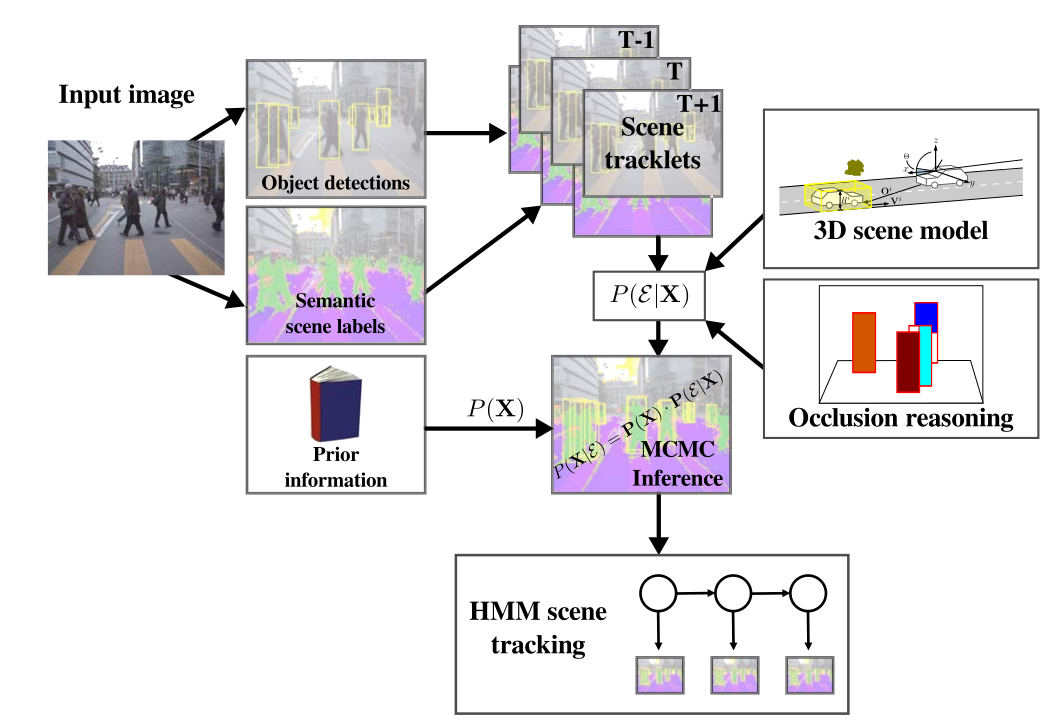
\includegraphics[width=0.5\textwidth]{graphics/wojek2013.png}

  Solve 3D localization in traffic scenes.

  Use semantic pixel labeling

  Use partial detectors for occlusion reasoning

  \pause
  But do not model traffic-scene interaction

  No traffic-traffic interaction
  % did exactly same way but we have better occlusion model because our
  % occlusion models are continous.
    
\end{frame}

\begin{frame}{\cite{Geiger_etal_2012} }
  % used stereo imagery and a restricted lane model that
  % reduce vehicle localization to a 1-D search on the lane.
  % 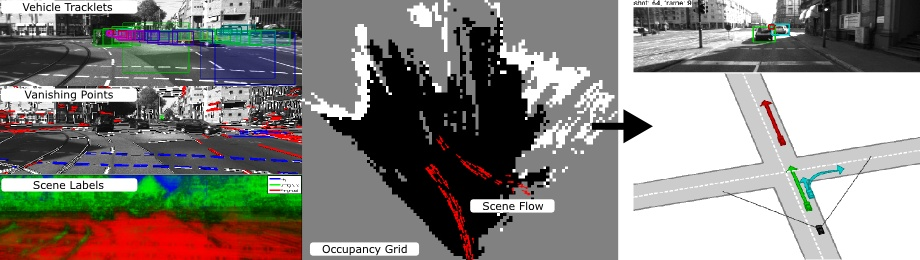
\includegraphics[width=\textwidth]{graphics/geiger_intersection_2012_1.jpg}\\

  Solve 3D localization in intersection scenes

  Model traffic-scene interaction by using lane information

  \pause
  But use stereo input 
  
  Lane model is too restrictive

  \begin{center}
    \begin{tikzpicture}
\providecommand{\imgwidth}{\textwidth}
      \path [use as bounding box,clip] (0.44\imgwidth,0) rectangle (0.73\imgwidth,3.5);
      \node [anchor=south west,inner sep=0] (img) at (0,0) {
      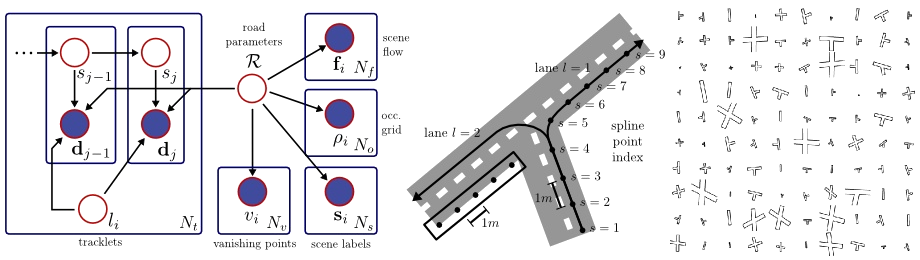
\includegraphics[width=\imgwidth]{graphics/geiger_intersection_2012_2.png}};
    \end{tikzpicture}
  \end{center}

    
\end{frame}

\begin{frame}{ \cite{Milan_etal_2014}}
  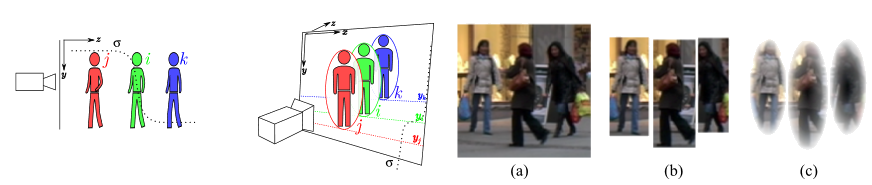
\includegraphics[width=\textwidth]{graphics/milan2014.png}
  % Use continuous occlusion model in multi-tracking framework but those are
  % just in 2D, our occlusion model is more principled and is in 3D.

  Solve tracking by detection using soft occlusion reasoning

  Model traffic-traffic interaction

  \pause
  But no traffic-scene interaction
  
  Also, occlusion model can be more principled and detailed
\end{frame}

\begin{frame}{What is missing?}
  \begin{columns}
    \begin{column}{0.5\textwidth}
      \visible<2->{Scope of improvement\\}
      \begin{itemize}
        \item Principled occlusion modeling      
        \item Flexible Traffic-Scene interaction       
        \item Traffic-traffic interaction            
      \end{itemize}
    \end{column}

    \begin{column}{0.5\textwidth}
      \visible<2->{
        Energies in our model\\
        \begin{itemize}
          \item {\coltrack Point tracks energy with occlusion modeling}
          \item {\collane Lane energy}
          \item {\colcol Collision energy}
        \end{itemize}
      }
    \end{column}
  \end{columns}
\end{frame}

